\chapter{Location of chips on breadboard}
\begin{figure}[H]
    \centering
    \includegraphics[width=0.8\textwidth]{images/locationOfChipsOnBreadboardUpdated.jpg}
    \caption{Location of chips on the breadboard}
    \label{fig:locationOfChipsOnBreadboard}
\end{figure}


\chapter{Colours of wires used}

\begin{table} [H]
\centering
\begin{tabularx}{0.8\textwidth} { X | X }
 
     \textsc{Colour of wire} & \textsc{Signal wire carrying} \\
     \hline
     \color{black}Black & \color{black}0V \\  
     \color{blue}Blue & \color{black} Binary data \\
     \color{brown}Brown & \color{black}-5V \\
     \color{orange}Orange & \color{black}Analogue Data / Control \\
     \color{purple}Purple & \color{black}Functional pins (eg, enable / reset) \\
     \color{red} Red & \color{black} +5V \\
     \color{yellow}Yellow & \color{black}Clock \\

\end{tabularx}
\end{table}

\chapter{Full schematic}
\label{app:fullSchematic}
\begin{figure}[H]
    \centering
    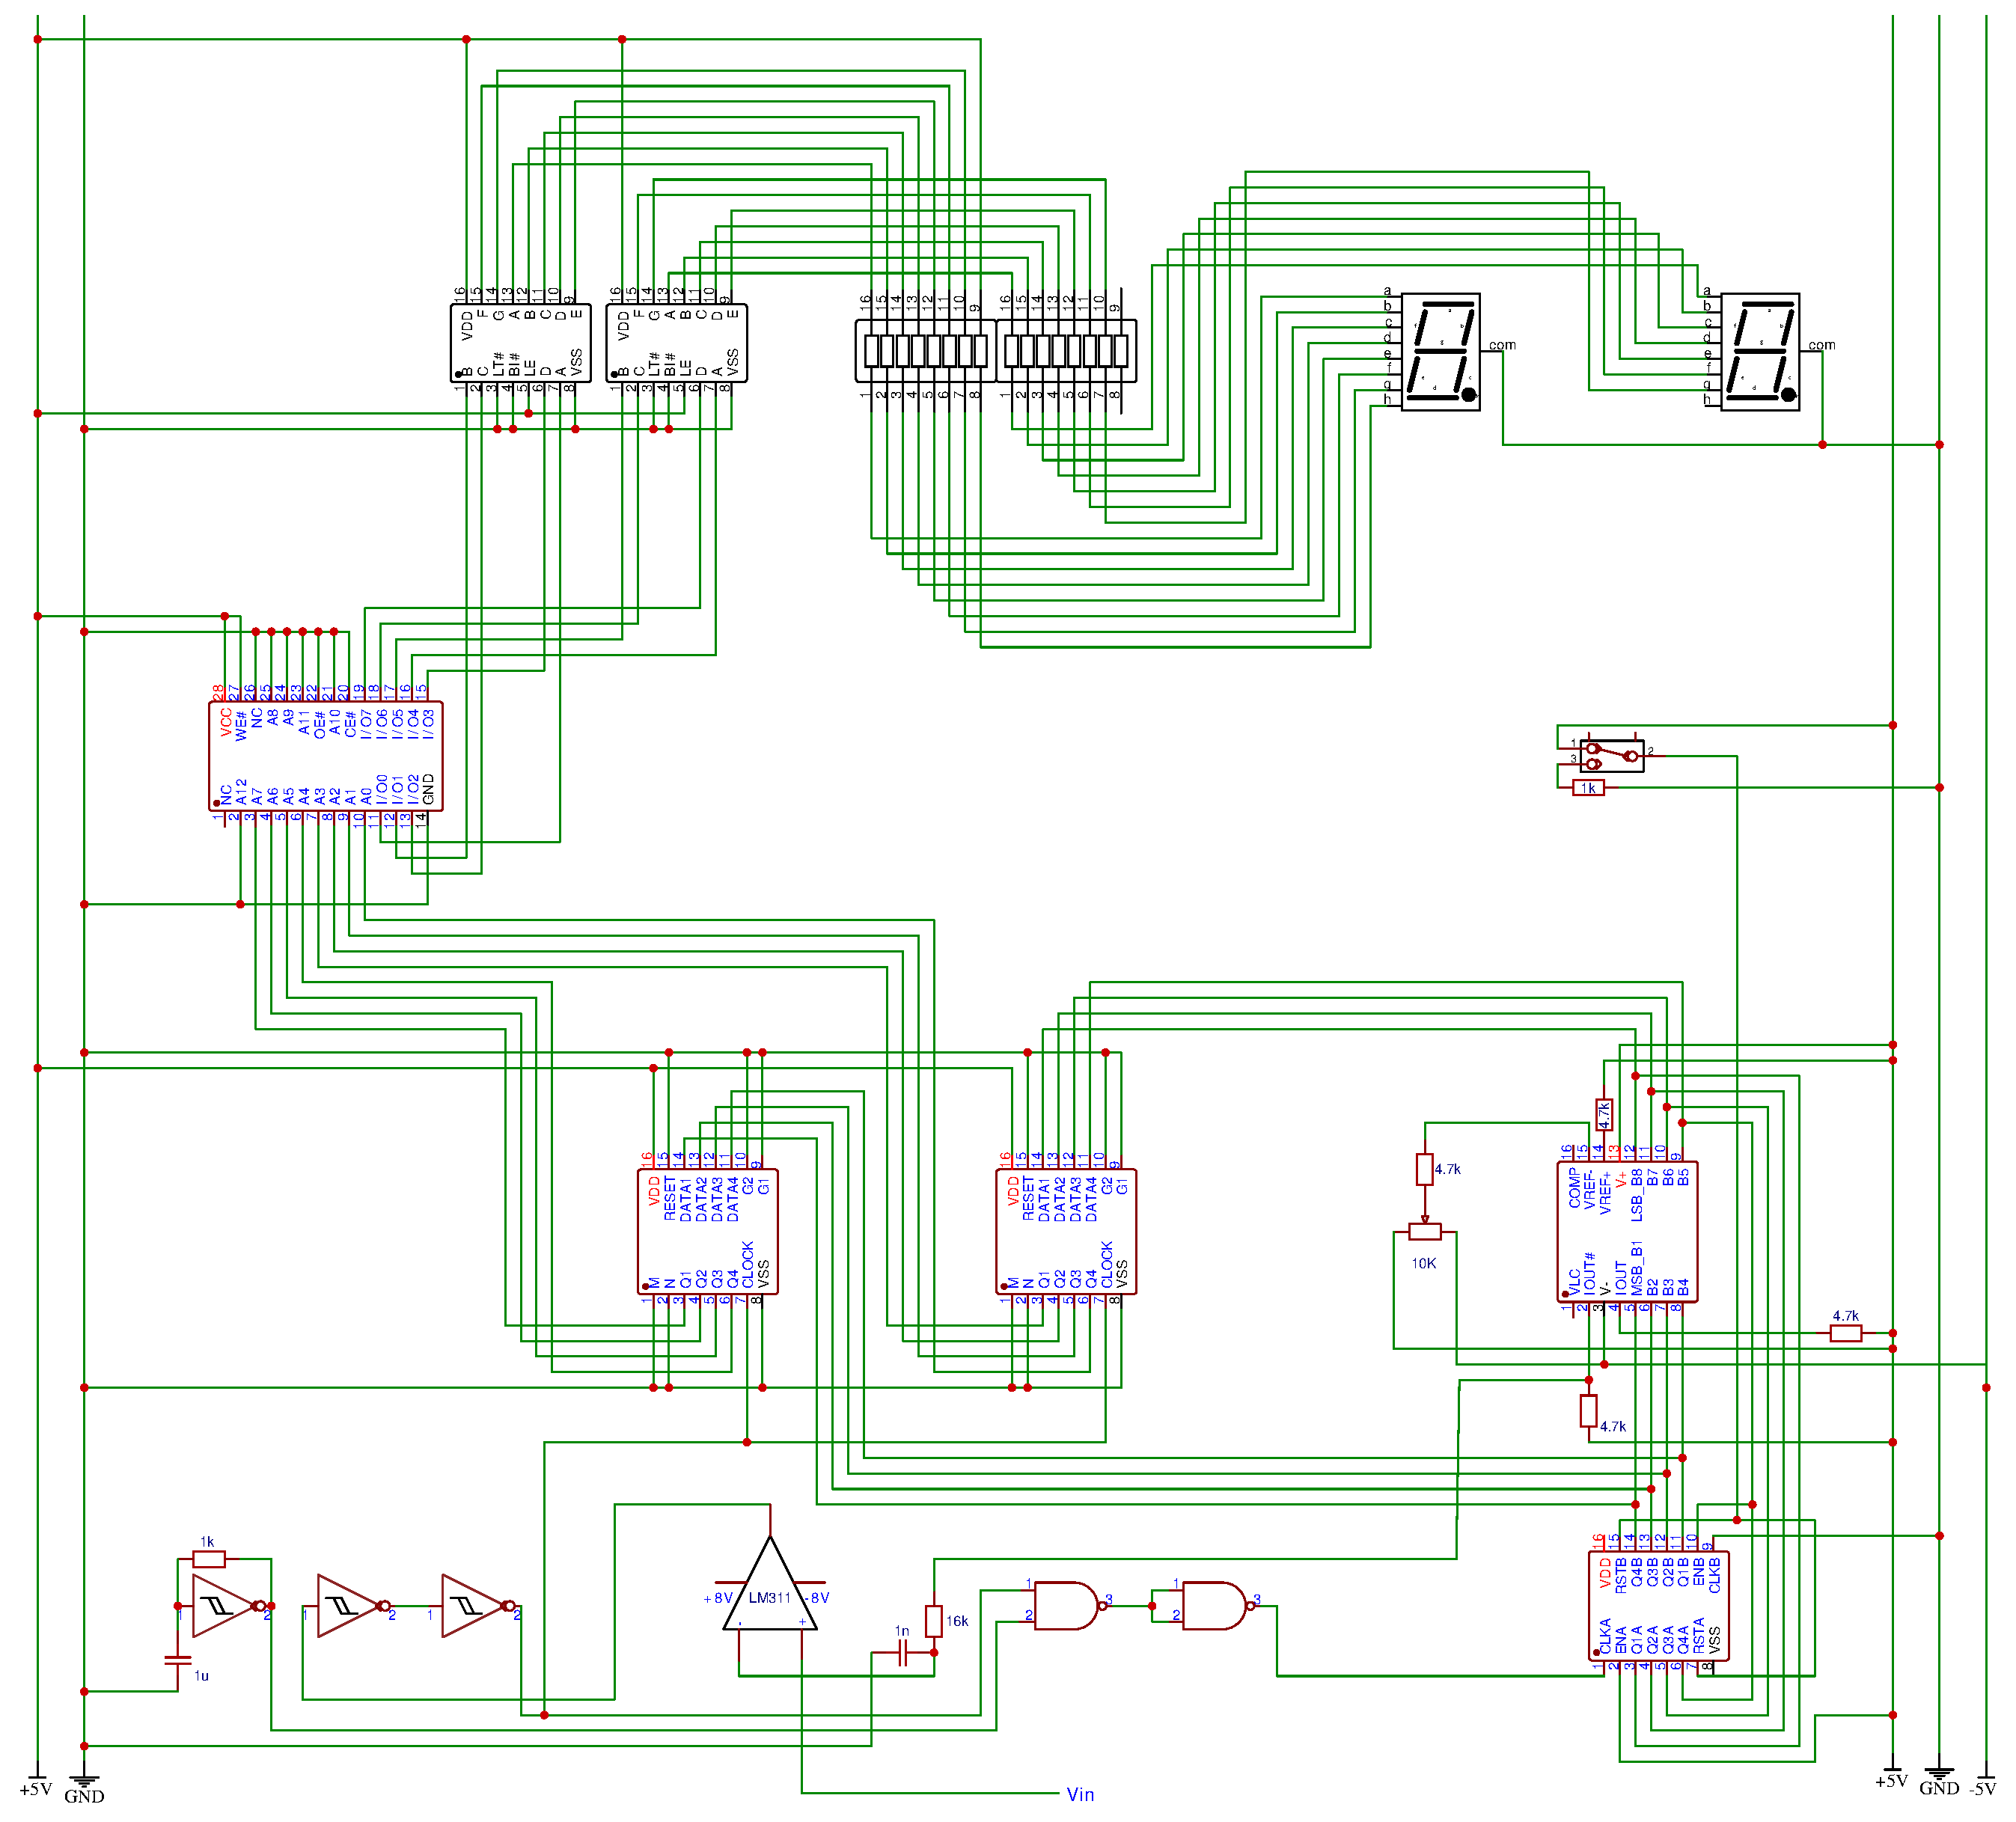
\includegraphics[width=\textwidth]{images/fullSchematic.pdf}
    \caption{Full Schematic}
    \label{fig:fullSchematic}
\end{figure}

\chapter{Final Physical Layout}
\begin{figure}[H]
    \centering
    \includegraphics[width=\textwidth, angle=270 ]{images/finalLayout.jpg}
    \caption{Final layout of the circuit}
    \label{fig:finalLayout}
\end{figure}




\chapter{Full Components list}
\section{Resistors}
\begin{itemize}
    \item 2 $220\Omega$ 8-way resistor packs
    \item 1 $380\Omega$ 
    \item 1 $1K\Omega$
    \item 4 $4.7K\Omega$
    \item 1 $10K\Omega$ rotary potentiometer
    \item 1 $10K\Omega$
    \item 1 $16K\Omega$
\end{itemize}

\section{Capacitors}
\begin{itemize}
    \item 7 $1\mu F$
    \item 1 $1nF$
\end{itemize}

\section{Integrated Circuit Chips}
\begin{itemize}
    \item 1 CD40106, Hex Schmitt Inverter, https://www.ti.com/lit/ds/symlink/cd40106b.pdf
    \item 1 LM311, Comparator, https://www.ti.com/lit/ds/symlink/lm311.pdf
    \item 1 CD4011, Quad NAND Gates, https://www.ti.com/lit/ds/symlink/cd4011b.pdf
    \item 1 CD4520, Dual Binary Up-Down Counter, https://www.ti.com/lit/ds/symlink/cd4520b.pdf
    \item 1 DAC0800LCN, 8-Bit Digital To Analogue Converter,\\ https://www.ti.com/lit/ds/symlink/dac0800.pdf
    \item 2 CD40706, 4-Bit D-Type Registers, https://www.ti.com/lit/ds/symlink/cd4076b.pdf
    \item 2 CD4511, BCD-To-7-Segment Latch Decoder Drivers,\\ https://www.ti.com/lit/ds/symlink/cd4511b.pdf
    \item 1 AT28C64B, 64K (8K x 8) Parallel EEPROM with Page Write and Software Data Protection, https://ww1.microchip.com/downloads/en/DeviceDoc/doc0270.pdf
\end{itemize}

\section{Other}
\begin{itemize}
    \item 1 Push-To-Make button
\end{itemize}

